%%%%%%%% ICML 2019 EXAMPLE LATEX SUBMISSION FILE %%%%%%%%%%%%%%%%%

\documentclass{article}

% Recommended, but optional, packages for figures and better typesetting:
\usepackage{microtype}
\usepackage{graphicx}
\usepackage{subfigure}
\usepackage{booktabs} % for professional tables
\usepackage{tikz} % for custom figures 
\usetikzlibrary{arrows,calc,fit, patterns}
\definecolor{blue}{rgb}{0.5,0.5,0.5}
\definecolor{tegreen}{RGB}{21,180,113}
\usetikzlibrary{arrows.meta}

% hyperref makes hyperlinks in the resulting PDF.
% If your build breaks (sometimes temporarily if a hyperlink spans a page)
% please comment out the following usepackage line and replace
% \usepackage{icml2019} with \usepackage[nohyperref]{icml2019} above.
\usepackage{hyperref}

% Attempt to make hyperref and algorithmic work together better:
\newcommand{\theHalgorithm}{\arabic{algorithm}}

% Use the following line for the initial blind version submitted for review:
%\usepackage{icml2019}

\usepackage{todonotes}
\newcommand{\cdavid}[1]{\todo[color=teal!60,inline]{D:#1}}
\newcommand{\ctim}[1]{\todo[color=green!60,inline]{T:#1}}
\newcommand{\chugo}[1]{\todo[color=red!60,inline]{H:#1}}
\newcommand{\crene}[1]{\todo[color=blue!60,inline]{R:#1}}
\newcommand{\cnat}[1]{\todo[color=orange!60,inline]{N:#1}}
\newcommand{\cte}[1]{\todo[color={rgb:red,32;green,185;blue,119},inline]{Te:#1}}
\newcommand{\te}[1]{\textcolor{rgb:red,32;green,185;blue,119}{Te:#1}}
\newcommand{\nat}[1]{\textcolor{orange}{N: #1}}

% If accepted, instead use the following line for the camera-ready submission:
\usepackage[accepted]{icml2019}

% The \icmltitle you define below is probably too long as a header.
% Therefore, a short form for the running title is supplied here:
\icmltitlerunning{Keys of Reinforcement Learning In Robot Visual Tasks}

\begin{document}

\twocolumn[
\icmltitle{Keys of Reinforcement Learning In Robot Visual Tasks}

% It is OKAY to include author information, even for blind
% submissions: the style file will automatically remove it for you
% unless you've provided the [accepted] option to the icml2019
% package.

% List of affiliations: The first argument should be a (short)
% identifier you will use later to specify author affiliations
% Academic affiliations should list Department, University, City, Region, Country
% Industry affiliations should list Company, City, Region, Country

% You can specify symbols, otherwise they are numbered in order.
% Ideally, you should not use this facility. Affiliations will be numbered
% in order of appearance and this is the preferred way.
\icmlsetsymbol{equal}{*}

\begin{icmlauthorlist}
\icmlauthor{XXX}{}
\end{icmlauthorlist}

% \begin{icmlauthorlist}
% \icmlauthor{XXX}{}
% \icmlauthor{Hugo Caselles-Dupr\'e}{equal,ensta,softbank}
% \icmlauthor{Timoth\'ee Lesort}{equal,ensta,thales}
% \icmlauthor{Te Sun}{ensta}
% \icmlauthor{Natalia D\'iaz-Rodr\'iguez}{ensta}
% \icmlauthor{David Filliat}{ensta}
% \end{icmlauthorlist}

% \icmlaffiliation{ensta}{Flowers Laboratory (ENSTA ParisTech, INRIA)}
% \icmlaffiliation{softbank}{AI Lab, Softbank Robotics Europe}
% \icmlaffiliation{thales}{Theresis Lab, Thales}

% \icmlcorrespondingauthor{Hugo Caselles-Dupr\'e}{caselles@ensta.fr}
% \icmlcorrespondingauthor{Timoth\'ee Lesort}{timothee.lesort@ensta.fr}
% \icmlcorrespondingauthor{Ren\'e Traor\'e}{rene.traore@ensta.fr}

% % You may provide any keywords that you
% % find helpful for describing your paper; these are used to populate
% % the "keywords" metadata in the PDF but will not be shown in the document
% \icmlkeywords{Machine Learning, ICML}

\vskip 0.3in
]

% this must go after the closing bracket ] following \twocolumn[ ...

% This command actually creates the footnote in the first column
% listing the affiliations and the copyright notice.
% The command takes one argument, which is text to display at the start of the footnote.
% The \icmlEqualContribution command is standard text for equal contribution.
% Remove it (just {}) if you do not need this facility.

%\printAffiliationsAndNotice{}  % leave blank if no need to mention equal contribution
% \printAffiliationsAndNotice{\icmlEqualContribution} % otherwise use the standard text.

\begin{abstract}
Reinforcement learning (RL) has emerged as a powerful tool to design navigation policies and control strategies for robots. However, how to design effective and efficient RL parameters is still an open question for various robotic tasks. In this study, we focus on the problem of teaching a robot to solve tasks with different configurations and find the keys to train the agent effectively. To achieve this, we designed a visual robot within a pushing box scenario and investigated the effects of parameters such as the visual encoder, policy network architecture, and training framework. In our work, we have fine-tuned the different hyperparameters (e.g., batch size, buffer size, learning rate) in the PPO algorithm to achieve the highest success rate for the task. We have also investigated if the training performance can be improved by using long short-term memory (LSTM), deeper convolutional neural networks, or imitation learning. Our results showed the feasibility of a learning-based controller and, therefore, served as a guideline and benchmark for implementing a learning-based controller for other similar tasks in real-life settings.
\end{abstract}

\section{Introduction}

% General context
There has been a growing interest in adopting artificial intelligence (AI) solutions in the perception, navigation, and control domains for robots, as they have been shown to be able to accomplish tasks better than humans. Among the AI algorithms, reinforcement learning (RL) \cite{kaelbling1996reinforcement} is a popular method that is used in this domain. Hence, we aim to investigate the effectiveness of RL in guiding and controlling a robot when performing a specific task with visual observations. Our goal is to develop a RL-based controller that can guide a robot to find a target and push it to the desired area by using visual data. Even though there are many RL algorithms that can be suitable for this application, we only consider the Proximal Policy Optimization (PPO) algorithm \cite{openai_ppo} as the benchmark. PPO has been a popular algorithm in this domain due to its state-of-the-art performance regarding adaptation capabilities in different tasks.

% Motivation
However, in most cases, designing suitable training schemes can be a painful process, with too many modules and parameters to be confirmed before training. For instance, there are various visual encoders, such as simple CNN, deeper CNN, ResNet-based CNNs \cite{he2016deepresidual}, etc. Besides, different policy neural network architectures also affect a lot of the performance of a RL controller. Moreover, to improve training sample efficiency, expert demonstrations are fused into some offline RL methods \cite{kober2010imitation}. Among these domains, variant combinations are still not clear to robot learning \cite{ravichandar2020recent}, which hinders the further development of RL-based controllers for robots. In this study, by using PPO as our RL algorithm, we comprehensively explore policy network architectures, different deeper convolutional neural networks, and imitation learning to achieve better results. As such, these investigations provide a design framework for robot learning before starting training without considering potential optimal solutions.


% \begin{figure}
%     \centering
%     \includegraphics[scale=0.2]{images/photo_real_life_two_tasks.png}
%     \caption{Having access to task 1 only first, and then task 2 only, we learn a single policy that solves two real-life navigation tasks using policy distillation and sim2real transfer.}
%     \label{fig:real_life_tasks}
% \end{figure}

% In our approach we aim to take advantage of simulations to create this scenario. We demonstrate %a successful attempt at 
% that deploying a policy in real-life which has continually learned two tasks in simulation is successful with our approach. 

% contributions
% Our contribution consists of applying two major paradigms for robotics in real life: a state representation learning approach for compact and efficient representation that facilitates learning a policy, and a policy that learns continually in a sequential manner. The approach is deployed in a real robot thanks to policy distillation and sim2real transfer. Furthermore, in opposition to most methods of RL, the solution we propose does not require a task indicator at test time. Indeed, information about the task to be solved can be found on a different color tag in the image.

Our contribution lies in exploring a synergy of diverse policy network architectures and deeper convolutional neural networks (CNNs), including ResNet-based models, to enhance the efficiency and effectiveness of RL-based controllers in visual tasks. We also investigate imitation learning compared to the PPO algorithm, boosting training sample efficiency and accelerating the learning process. This innovative combination enables our RL controller to adeptly guide robots in identifying and manipulating targets, crucially without the need for explicit task indicators during testing. Our work not only provides a robust, efficient RL solution for complex visual robotic tasks but also simplifies the preliminary design process, offering a clear framework for configuring RL controllers in real-world applications.

%framework
In the following section, we will formulate our RL problem. By using this framework, we have done the following: 1) tune the PPO’s hyperparameters to achieve optimal results; 2) investigate if the results can be improved by adding LSTM layers to our models; 3) compare the results achieved by convolutional neural network variants of different architectures; 4) observe if the results can be improved by giving human demonstrations to the models (i.e., imitation learning). The rest of the article is structured as follows. Section \ref{ref:relatedwork} introduces robot learning with RL; Sec.\ref{ref:experiments} details the robotics settings and tasks performed; Sec.\ref{ref:methods} describes the methods utilized; Sec. \ref{ref:results} presents the results and discussion; Sec. \ref{ref:conclusion} concludes with future insights from our simulation experiments.

\section{Related Work}
\label{ref:relatedwork}
The integration of RL in robot learning has been a burgeoning area of research, driven by the need for adaptive and intelligent robotic systems. A significant contribution in this field has been the application of Deep RL (DRL). For instance, Levine et al. \cite{levine2016end} demonstrated the effectiveness of DRL in end-to-end training of robotic systems for complex tasks like manipulation and grasping, using raw pixel data as input.

Another notable advancement is the use of RL in robotic navigation and control. Tai and Liu \cite{tai2017virtual} explored how mobile robots could effectively navigate in complex environments using deep Q-networks, showcasing the potential of RL in real-world applications. Similarly, Ender et al. \cite{cetin2019drone} applied RL for robot navigation, specifically focusing on obstacle avoidance using convolutional neural networks (CNNs), setting a precedent for aerial robotics.

In the realm of multi-robot systems, Matignon et al. \cite{matignon2012coordinated} and Foerster et al. \cite{foerster2016learning} have made significant contributions. They explored the dynamics of cooperative and competitive behaviors among robots, using RL to facilitate effective strategies for tasks like pursuit-evasion games, highlighting the adaptability of RL in multi-agent scenarios.

The integration of imitation learning with RL has also gained traction. For example, studies by Nair et al. \cite{nair2018overcoming} have shown how imitation learning can be utilized to bootstrap the training process in RL, enhancing the learning efficiency in robotic manipulation tasks.

Moreover, the development of sample-efficient RL algorithms has been crucial for practical robotics applications. Haarnoja et al. \cite{haarnoja2018soft} introduced Soft Actor-Critic (SAC), an algorithm that optimizes policy in an entropy-augmented setting, demonstrating significant improvements in sample efficiency and robustness in robotic control tasks.

Finally, the concept of sim-to-real transfer in RL, where policies are trained in simulated environments and then transferred to real-world scenarios, has been a key area of research. Rusu et al. \cite{rusu2017sim} and James et al. \cite{james2019sim} have made substantial contributions in this area, showing how policies developed in simulated environments can be effectively adapted to physical robots, overcoming the challenges posed by real-world complexities.

However, before transferring the trained policy to a real robot, a fine-tuned model is required, which has not been fully investigated.


%We pose the question of How can one agent learn 2 tasks sequentially and at test time, be able to solve each task without forgetting? We want to use a unique "brain" for the agent, i.e. have a scalable solution (not a multi-head network as for instance it is used in Progressive Nets \cite{rusu2016progressive}.
%\nat{were task indicator is given?confirm and indicate}).

\section{Problem Formulation}\label{ref:experiments}
The key components in a RL problem include: the state \( s \), the agent, the action \( a \), the reward \( r \), and  the environment. In our system, the agent is an RL-based robot, which receives the state \( s \) as input and produces an action \( a \) following a policy \( \pi \). The action space is defined by discrete movements tailored to guide the robot towards a box and subsequently push it to a designated \textit{Target Area}, as shown in Figure 1.

The agent's objective is to learn a policy \( \pi_\theta(s,a) \) that prescribes the optimal action \( a \) for each state \( s \). In deep RL, this policy is represented by a neural network with parameters \( \theta \), which are trained to select the most favorable action for any given state.

Our simulated environment is a simplified 2D representation of a room, consisting of a robot with forward RGB camera and a box, the latter serving as the target object. The layout of the room remains unchanged across episodes, except for the box's position, which is randomized each episode. The agent is further challenged by variable lighting conditions that shift after every episode, testing its adaptability.

Interactions of the robot with the environment, such as advancing towards and maneuvering the box, induce changes within the environment, evidenced by alterations in the robot's position and orientation. These modifications are computed utilizing the robot's equations of motion, accounting for the cumulative influence of thrust and body angular rates on the robot's dynamics. The \textit{Visual Observation} in the figure underscores the robot's perception capacity, pivotal for recognizing the environment's state and determining the subsequent action.


\subsection{Observation Space}
The state \( s \) encapsulates a representation of the current status of the environment, serving as the critical input to the agent. It comprises significant features that enable the agent to exploit the environment and make informed decisions. Within our application, the observed state is only a visual input from the robot's onboard camera.

\subsection{Action Space}
The action space defines the set of all possible actions the agent can take. In the context of our robotic application, this action space includes six discrete actions, namely \{forward, back, turn-left, turn-right, left, right\}, aimed at navigating the robot in the environment towards the achievement of its goal.

\subsection{Reward Functions}
The reward function provides feedback to the agent upon executing an action, resulting in environmental changes. The reward is structured as follows: a positive reward of \( +5 \) is allocated when the robot successfully reaches the target, incentivizing the discovery of the target. A negative reward of \( -5 \) is imposed if the robot move out of area, deterring the agent from engaging in collision-prone behavior.
Given that these rewards are dispensed solely at the terminal step, the agent often experiences a period with no reward, culminating in a sparse reward function. To mitigate the associated learning challenges, an additional penalty given each step to encourage agent to finish task quickly, namely $-1 / MaxStep$.

\subsection{Learning Objective}
The overarching aim for the agent is to adjust the parameters \( \theta \) in the policy \( \pi_\theta(s,a) \) to maximize the cumulative reward obtained within an episode, thus steering the robot efficiently towards the target.

\begin{figure}[!tb]
\centering
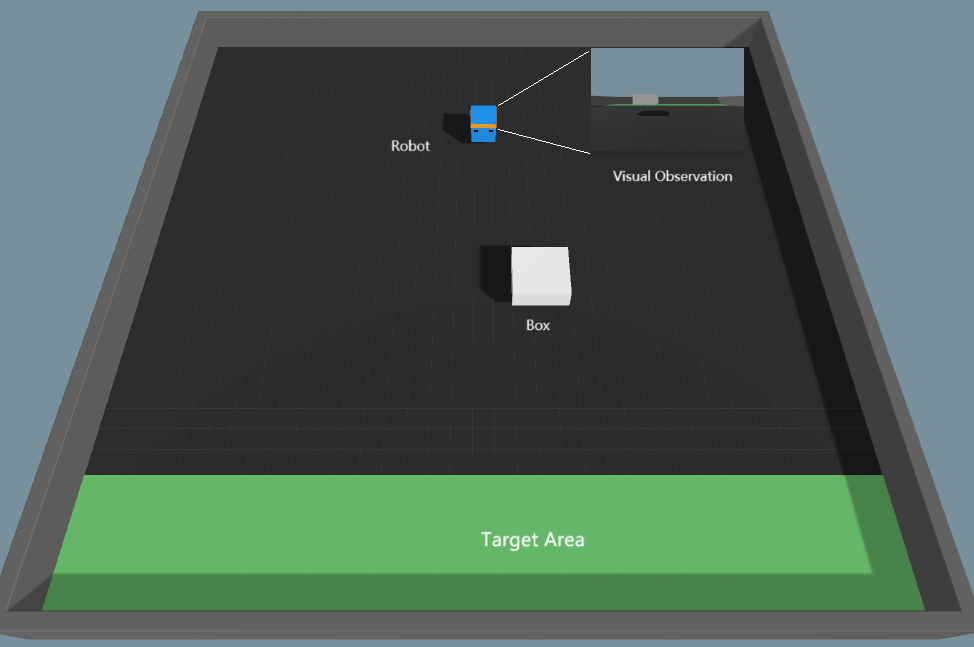
\includegraphics[width=0.45\textwidth]{images/push.png}
\caption{Pushing box task with visual perception}
\end{figure}


\section{Methods}
\label{ref:methods}
%\chugo{Manque une intro qui raconte a quoi sont liées ces méthodes.}
\subsection{PPO Baseline}
\label{subsec:ppo}
%\chugo{Decrire comment on génére le dataset on-policy.}
Unlike many on-policy RL algorithms, PPO does not need to discard the old experiences and collect a new batch of experiences after each policy update. PPO allows the policy (i.e., the neural network) to be updated multiple times using different batches of experiences. This greatly reduces the training time as fewer data are needed to be collected each time. To further speed up the training, we have used six parallel environments that the agent can interact with. The agent can take different actions in these environments and collect different sets of experiences in parallel. Aside from speeding up the data collection, parallel environments reduce the correlation in the dataset. 
Besides improving the time efficiency, the PPO algorithm is designed to have a more stable training. This is done by adding a new constraint that limits how much the updated policy can differ from the old policy [1].
Due to the above-mentioned benefits, PPO is well suited for our complex application. 

We have chosen Proximal Policy Optimisation (PPO) algorithm to train the agent as PPO has achieved state-of-the-art performance in many similar control problems [1]. PPO uses the actor-critic framework shown in figure 2 [2]. The critic is a value function estimator and uses a deep learning model to predict the state-value $V(s)$ from the state s. The state-value $V(s)$ is the expected value of the discounted cumulative reward by starting at state (s). In essence, the state-value $V(s)$ measures how good it is to be in state (s). The actor derives the policy $\pi_\theta(s,a)$ which maps the optimal action (a) to each state (s). For a given state (s), the actor uses a deep learning model to predict a continuous probability distribution over the action space. When the actor is trained successfully, the optimal action will receive the highest probability.

In our implementation, the actor and critic have the same deep learning model architecture, as shown in figure 3. The image component of the state is processed by a convolutional neural network (CNN) variant while the vector component of the state is fed into a 2-layer neural network (NN). The extracted features from the image and vector are then combined and fed into another 2-layer neural network for prediction. The actor predicts the probability distribution over the action space while the critic predicts the state-value \( V(s) \). At the start of the training, the actor and critic neural networks are initialised with random weights. By taking random actions, the agent collects experiences that are stored in the form: \( \langle s_t, a_t, r_t, s_{t+1} \rangle \). In this form, the agent takes action \( a_t \) at state \( s_t \). As a result, the agent receives a reward \( r_t \) and transits to a new state \( s_{t+1} \).

For each experience \( \langle s_t, a_t, r_t, s_{t+1} \rangle \), we can use the critic to find \( V(s_t) \) and \( V(s_{t+1}) \) for \( s_t \) and \( s_{t+1} \) respectively. If the critic neural network is a perfect estimator of the state-value \( V(s) \), the following equation will be true:
\begin{equation}
V(s_t) = r_t + \gamma V(s_{t+1})
\end{equation}
where \( \gamma \) is the discount factor and \( r_t \) is obtained from the agent’s experience. By rearranging, we will obtain:
\begin{equation}
r_t + \gamma V(s_{t+1}) - V(s_t) = 0
\end{equation}

\begin{table}[!tb]
\centering
\caption{Hyperparameters used for PPO.\label{tb:hyper}}
\begin{tabular}{l|l}
\toprule
\textbf{Hyperparameter} & \textbf{Value} \\
\hline
Discount factor & 0.99 \\
Batch size & 1024 \\
Buffer size & 10240 \\
Learning rate & 0.0003 \\
Beta & 0.01 \\
Epsilon & 0.2 \\
Lambda & 0.95 \\
Learning rate schedule & Linear schedule \\
Training episodes & 5 million\\
\bottomrule
\end{tabular}
\label{table:hyperparameters}
\end{table}

\begin{table}[!tb]
\centering
\caption{Characteristics of pre-collected human experiences}\label{table:human-experiences}
\begin{tabular}{l|l}
\toprule
\textbf{Characteristic} & \textbf{Value} \\
\hline
Duration of recording & ~1 hour \\
Number of steps recorded & 35050 \\
Number of episodes recorded & 528 \\
Mean reward & 4.492926 \\
\bottomrule
\end{tabular}
\end{table}

Due to estimation error in the critic neural network, the right-hand side of the equation is equal to a non-zero value \( \delta_t \). Hence,
\begin{equation}
r_t + \gamma V(s_{t+1}) - V(s_t) = \delta_t
\end{equation}
The non-zero quantity \( \delta_t \) is the error of the critic’s estimation of \( V(s_t) \) and is also referred to as the temporal difference error (TD error). We use the TD error as the loss function for our critic neural network and drive this error to zero using gradient descent. For the same experience \( \langle s_t, a_t, r_t, s_{t+1} \rangle \), the actor neural network receives \( s_t \) as input and outputs the probability distribution over the action space. The following equation can be derived:
\begin{equation}
\delta_t = Q(s_t, a_t) – V(s_t)
\end{equation}
Thus, the TD error \( \delta_t \) also measures how good it is to take action \( a_t \) at state \( s_t \). More specifically, the difference \( Q(s_t, a_t) – V(s_t) \) shows how good \( a_t \) is compared to the average action in state \( s_t \). If the TD error \( \delta_t \) is positive (i.e., \( Q(s_t, a_t) > V(s_t) \)), the action \( a_t \) is favourable at \( s_t \). Hence, the actor neural network will tune its weight such that the policy will increase the probability of \( a_t \) at \( s_t \). Conversely, a negative TD error \( \delta_t \) (i.e., \( Q(s_t, a_t) < V(s_t) \)) shows that the action \( a_t \) is not favourable at \( s_t \). Hence, the actor neural network will tune its weight such that the policy will decrease the probability of taking action \( a_t \) at \( s_t \).

In summary, the TD error \( \delta_t \) determines the direction and magnitude that the deep learning model should adjust its weights towards. In practice, we use multiple experiences (i.e., batch size $>$ 1) to find an average \( \delta_t \) which is used to update the weights in Actor and Critic. This keeps the training stable.

We have implemented the environment and trained the agent using the Unity Ml-Agents Toolkit \cite{juliani2020}. The following table shows the hyperparameters that we have used for PPO. These hyperparameters are held constant as we examine the use of Long Short-Term Memory (LSTM), CNN variants (e.g., Resnet), and imitation learning for our deep learning model.



\subsection{Variation Studies}
\subsubsection{Long Short-Term Memory}
In addition to memoryless neural networks (refer to Figure 3), we have explored the addition of memory to the actor and critic neural networks by integrating Long Short-Term Memory (LSTM) layers. Similar to recurrent neural networks, LSTM layers learn to combine features from both current and past inputs \cite{hochreiter1997lstm}. However, LSTM's additional gates allow for more flexible mixing of current and past features, enabling it to retain older information more effectively. This potentially leads to richer feature extraction that can be utilized by the prediction layer. In our implementation, the LSTM model processes inputs from time \( t \) to \( t-63 \).

\subsubsection{CNN Variants}
Beyond the simple 2-layer CNN used in the actor and critic model, we investigated the effectiveness of other CNN variants, namely Nature CNN and Resnet, in enhancing training performance. Nature CNN, with three convolutional layers, is a larger network compared to the simple 2-layer CNN \cite{mnih2015humanlevel}. Among these variants, Resnet is the most extensive network. Its skip connections help overcome the vanishing gradient problem associated with deeper networks \cite{he2016deepresidual}. While Nature CNN and Resnet have more layers, potentially leading to richer feature extraction, their larger size also implies longer training times.

\subsubsection{Imitation Learning}
Our approach also considers the potential benefits of incorporating pre-collected human experiences into the training of deep learning models. The characteristics of our pre-collected human data are shown in Table \ref{table:human-experiences}. In our implementation, the agent is trained using both the pre-collected human experiences and its own experiences for 1,000,000 steps. After this period, the agent continues its training solely on its experiences. This strategy allows the agent to learn beyond the provided data and potentially surpass human performance. The performance of our pre-collected human experiences also serves as a benchmark for evaluating our deep learning models, where a well-trained model should achieve a mean reward close to or exceeding 4.492926.

\section{Results and Discussions}\label{ref:results}
\subsection{Usefulness of LSTM}
In our first experiment, we investigated the usefulness of LSTM in improving the training performance. From Figure \ref{fig2}, we observed that both models trained successfully. The cumulative reward for both models increased and converged at approximately 2.5, and the episode length (i.e., the number of steps taken per episode) decreased, converging at around 350. We found no significant improvement in training performance when using LSTM. In our problem formulation, we explicitly provided past information to our deep learning model, allowing the non-LSTM model to access past information. This suggests that our problem formulation already retained the required past knowledge for our deep learning models, making the use of LSTM unnecessary. Although LSTM did not worsen training performance, its significantly longer training time suggests avoiding its use.

\begin{figure}[!tb]
\centering
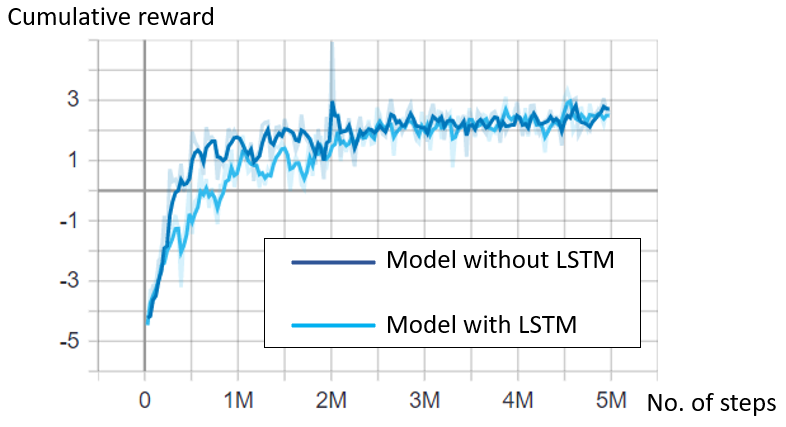
\includegraphics[width=0.5\textwidth]{images/fig1.png}
\caption{Comparison of training performance (cumulative reward) between model without LSTM and model with LSTM}\label{fig2}
\end{figure}

% \begin{figure}[h]
% \centering
% \includegraphics[width=0.8\textwidth]{figure5.png}
% \caption{Comparison of training performance (episode length) between model without LSTM and model with LSTM}
% \end{figure}

\subsection{Usefulness of Deeper CNN Variants}
In our second experiment, we explored whether training performance could be improved using deeper convolutional neural networks. As shown in Figure \ref{fig3}, the deeper models (i.e., nature CNN and Resnet) worsened the training performance. The nature CNN’s cumulative reward converged at a lower value (~2) compared to the simple 2-layer CNN model (~2.5), and its episode length converged at a higher value (~450) than the simple CNN model (~350). Among the three models, Resnet performed the worst with a significantly lower cumulative reward and a longer episode length. While deeper networks have the potential to learn richer features, they are more challenging to train. To improve training performance, it may be necessary to increase the number of training steps and experiment with different hyperparameters. The hyperparameters in Table 1 were insufficient for deeper models to outperform the simple CNN model.

\begin{figure}[h]
\centering
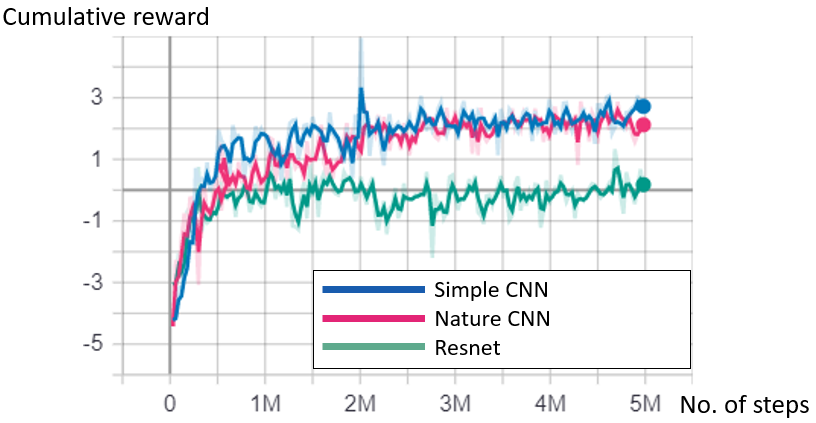
\includegraphics[width=0.5\textwidth]{images/fig2.png}
\caption{Comparison of training performance (cumulative reward) between CNN variants}\label{fig3}
\end{figure}

% \begin{figure}[h]
% \centering
% \includegraphics[width=0.8\textwidth]{figure7.png}
% \caption{Comparison of training performance (episode length) between CNN variants}
% \end{figure}

\subsection{Usefulness of Imitation Learning}
In our final experiment, we assessed whether imitation learning could enhance training performance. By adjusting the number of training steps to 1,000,000, we sought optimal results with imitation learning. Figure \ref{fig4} shows the training results with imitation learning. The training performance did not improve significantly with imitation learning, and the model with imitation learning underperformed compared to human demonstrations, achieving a converged cumulative reward of 2.8 against the human demonstration score of 4.492926.

\begin{figure}[h]
\centering
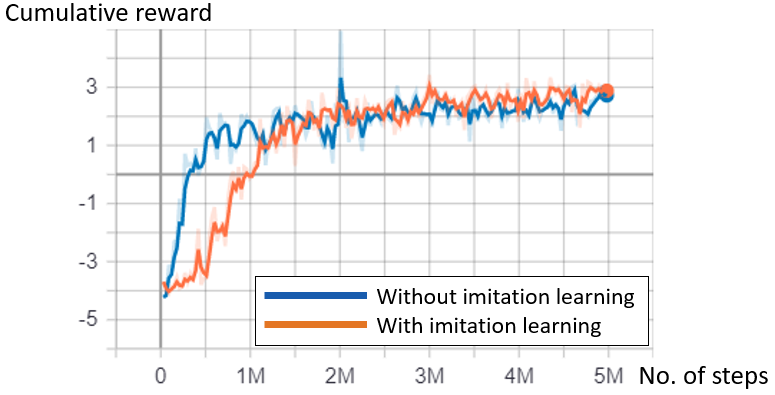
\includegraphics[width=0.5\textwidth]{images/fig3.png}
\caption{Comparison of training performance (cumulative reward) between model without imitation learning and model with imitation learning}\label{fig4}
\end{figure}

% \begin{figure}[h]
% \centering
% \includegraphics[width=0.8\textwidth]{figure9.png}
% \caption{Comparison of training performance (episode length) between model without imitation learning and model with imitation learning}
% \end{figure}

\section{Conclusions} \label{ref:conclusion}
In our work, we have developed a RL environment using the Unity Machine Learning Agents Toolkit. We formulated the key elements (State, Agent, Action, Reward, Environment) of our RL problem and trained our agent using the PPO algorithm. In addition to tuning the hyperparameters for PPO, we examined the use of LSTM, deeper CNN variants, and imitation learning to improve training performance.

Based on the hyperparameters in Table 1, our results indicate that neither LSTM nor deeper CNN variants improved the training performance. The relatively simpler memoryless model shown in Figure 3 achieved moderately good training performance in a significantly shorter time. Therefore, we recommend continuing with this simpler model while experimenting with other hyperparameters. 

Imitation learning also showed no significant improvement using our parameters and did not outperform the human demonstrations. Further experimentation with other hyperparameters is necessary to meet or exceed this benchmark performance.

% \subsection{Learning on one task}
% \label{subsec:oneTask}

% \usetikzlibrary{arrows}
\usetikzlibrary{decorations.markings}
\newcommand{\mygrid}{\tikz{\draw[step=0.5cm] (0,0)  grid (0.5,1.5);}}

\begin{figure}[ht!]
\centering

\resizebox{0.45\textwidth}{!}{%   % line to set size of the whole image
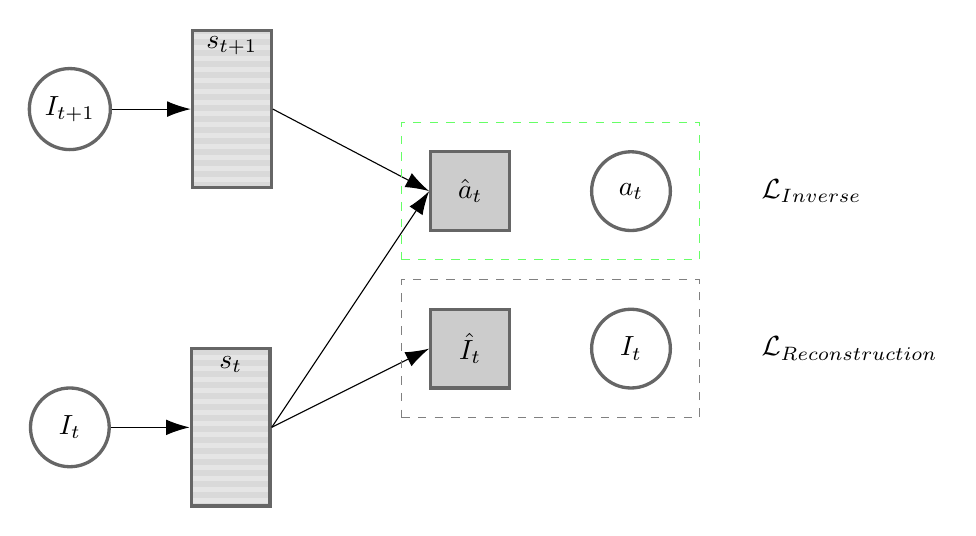
\begin{tikzpicture}[
roundnode/.style={circle, draw=black!60, fill=green!0, very thick, minimum size=10mm},
roundnode2/.style={circle, draw=black!60, fill=black!20, very thick, minimum size=10mm},
squarednode_st/.style={rectangle, draw=black!60, fill=green!20, very thick, minimum size=10mm},
squarednode/.style={rectangle, draw=black!60, fill=black!20, very thick, minimum size=10mm},
squarednode_st2/.style={rectangle, draw=black!60, very thick, minimum width=10mm, minimum height = 2cm},
invisible/.style={rectangle , draw=black!0, fill=green!0, very thick, minimum size=10mm},
squarednode_img/.style={rectangle, draw=black!60, fill=black!20, very thick, minimum size=10mm},
%grid_node/.style={minimum size=.5cm-\pgflinewidth, outer sep=0pt},
%model/.style={trapezium angle=60, minimum width=50mm, draw, thick, label=above:8cm, label=below:16cm, label=right:8cm, label=left:8cm}
container_AE/.style={draw, rectangle, draw=green!60, dashed, inner sep=1em},
container_Inv/.style={draw, rectangle, draw=blue, dashed, inner sep=1em},
]


%Nodes

%first column
\node[invisible]        (base)        {};
\node[invisible]        (base2)        [above=of base] {};

\node[invisible]        (obs)        {};
\node[invisible]        (obs2)        [above=of obs] {};

\node[roundnode]        (hidden_obs2)        [on grid,above=of base2] {$I_{t+1}$};
\node[roundnode]        (hidden_obs)        [on grid,below=of base] {$I_t$};
\node[invisible]        (hidden_obs3)        [on grid,above=of base] {};

%Second column
%\node[squarednode_st]      (state)        [right=of obs]{$s_t$};

%\node[rectangle, draw, inner sep=0] {\mygrid}  (state) [right=of obs];

\node[invisible]        (hidden_state)        [right=of hidden_obs3,draw] {};
\node[invisible]        (hidden_state)        [on grid,right=of hidden_state,draw] {};

\node[squarednode_st2] (anode) [right=of hidden_obs,draw, pattern=horizontal lines light gray]{};
%\node[squarednode_st] (state) [on grid,above=of anode,draw, pattern=checkerboard light gray]{};
\node[] (label) [on grid, above=0.8cm of anode]{$s_{t}$};


\node[squarednode_st2] (anode2) [right=of hidden_obs2,draw, pattern=horizontal lines light gray]{};
%\node[squarednode_st] (state2) [on grid,above=of anode2,draw, pattern=checkerboard light gray]{};
\node[] (label2) [on grid, above=0.8cm of anode2]{$s_{t+1}$};


% third column
% \node[squarednode]        (recon_rew)        [right=of hidden_state,draw, pattern=horizontal lines light gray] {$\hat{r}_t$};

\node[invisible]        (center3)        [right=of hidden_state] {};

\node[squarednode]        (recon_act)        [on grid, above=of center3, draw] {$\hat{a}_t$};
\node[squarednode]        (recon_img)        [on grid,below=of center3,draw] {$\hat{I}_t$};


% forth column
\node[roundnode]        (img)        [right=of recon_img,draw] {$I_t$};
% \node[roundnode]        (rew)        [right=of recon_rew,draw] {$r_t$};
\node[roundnode]        (act)        [right=of recon_act,draw] {$a_t$};

% fifth column
\node[invisible]        (L_img)        [right=of img,draw] {$\mathcal{L}_{Reconstruction}$};
% \node[invisible]        (L_rew)        [right=of rew,draw] {$\mathcal{L}_{Reward}$};
\node[invisible]        (L_act)        [right=of act,draw] {$\mathcal{L}_{Inverse}$};


% arrows

\draw[-{Latex[length=3mm,width=2mm]}] (hidden_obs.east) -- (anode.west);
\draw[-{Latex[length=3mm,width=2mm]}] (hidden_obs2.east) -- (anode2.west);

% \draw[-{Latex[length=3mm,width=2mm]}, dashed] (anode.east) -- (recon_rew.west);
% \draw[-{Latex[length=3mm,width=2mm]}, dashed] (anode2.east) -- (recon_rew.west);

\draw[-{Latex[length=3mm,width=2mm]}] (anode2.east) -- (recon_act.west);
\draw[-{Latex[length=3mm,width=2mm]}] (anode.east) -- (recon_act.west);

\draw[-{Latex[length=3mm,width=2mm]}] (anode.east) -- (recon_img.west);


% containers
%\node[container_Inv, fit=(recon_rew) (rew)] (ae) {};
\node[container_AE, fit=(recon_act) (act)] (fwd) {};
\node[container_Inv, fit=(recon_img) (img)] (ae) {};

\end{tikzpicture}
}

\caption{\textit{SRL Combination} model: combines the prediction of an image $I$'s reconstruction loss and an inverse dynamic model loss in a state representation $s$. Arrows represent inference, dashed frames represent losses computations, rectangles are state representations, circles are real observed data, and squares are model predictions, $t$ represents the timestep}

\label{fig:split-model}
\end{figure}

% %\cdavid{If we keep talking about sim2real, you should say here that its trained in simulation with data augmentation. By the way, saying that we train in simulation reduces a bit the interest of continual learning. If we are able to simulate everything, why bother learning incrementally and not simulating the two tasks simultaneously ?}
% %\ctim{on peux imaginer que lorsqu'une nouvelle tache est à apprendre dans la vrai vie, on fait appelle à la simulation pour accélerer. d'après moi, ca ne veut pas dire que la simulation a nécessairement accés aux taches futures et ça permet d'apprendre de facon continue.}

% %intro
% Each task $i$ is learned following to procedure we describe here.
% %generation of D_R
% First, as we use an SRL approach, we need to learn a state representation encoder.
% We sample data from the environment $Env_i$ (where $i$ refers to the task) with an agent guided by a random policy. We call this dataset $D_{Random,i}$.
% % learning SRL_t
% $D_{Random,i}$ is then used to train an SRL model composed of an inverse model and an auto-encoder. This architecture is inspired from \cite{raffin2019decoupling}, and illustrated in Fig. \ref{fig:split-model}.
% %\ctim{a figure with the SRL model would be nice}

% %David : maybe not useful to make 2 figures
% %\begin{figure*}
% %\includegraphics[scale=0.3]{images/step1_explained.png}
% %\caption{Focus on step 1 at the top. We first learn a representation model for the environment. Then using RL, we learn a policy that takes the learned features as input. Once the policy is finished training, we generate an on-policy dataset for distillation: sequences of observations and action probabilities associated.}
% %\end{figure*}


% \begin{figure*}
% \centering
% \includegraphics[width=.9\textwidth]{images/overview.png}
% \caption{Summary of the experimental setup. Step 1 and 2 correspond to learning policies for task 1 and 2, and using those to create distillation datasets. Step 3 is the distillation of the two policies into a single policy which can be deployed in simulation and on the real robot.}
% %\bigbreak
% \label{fig:overview}
% \end{figure*}


% % learning pi_t
% Once the SRL model is trained, we use it's encoder $E_i$ to provide with features for learning a RL policy $\pi_i$ with the model $M(\theta)$ ($\theta$ represents the model parameters).
% % generation of Dpi_t
% Once $\pi_i$ is learned, we use it to generate sequences of on-policy observations with associated actions, which will eventually be used for distillation (Fig. \ref{fig:overview}, right). We call this the distillation dataset $D_{\pi i}$. We generate $D_{\pi i}$ the following way: we randomly sample a starting position and then let the agent generate a trajectory. At each step we save both the observation and associated action. We stop the sequence when enough reward is gathered (see Section \ref{ref:experiments}).% N early stopping? any programmatic rule particularly used?

% From each task is only kept the dataset $D_{\pi_i}$. As soon as we change task, $D_{Random,i}$ and $Env_i$ are not available anymore.
% %\cdavid{and $D_{Random,i}$ ?}

% In our setting, in order to decrease training time, we generate $D_{Random,i}$ in simulation and learn $\pi_i$ also in simulation. However, at the end of $T$ tasks, $\pi_{D_0,...,D_{T-1}}$ are tested in a real robot. In order to pass the reality gap, the datasets generated are augmented with different luminosity variations.

% \subsection{Learning continually}
% \label{subsec:continual_learning}

% To learn continually we use a distillation algorithm \cite{rusu2015policy}. Once we learned several tasks, we can aggregate the distillation datasets $D_{\pi_i}$ and distill the knowledge into a new model $M_Di(\theta')$ to produce a single flexible %monolithic 
% policy (Fig. \ref{fig:overview}, right). $\theta'$ are the parameters of the distillation model.

% The distillation consists in learning in a supervised fashion the action probability associated to an observation at a timestep $t$. Each dataset $D_{\pi_i}$ allows to distill the policy $\pi_i$ into a new network. We name the distilled policy $\pi_{D_i}$. With the aggregation of several distillation datasets, we can distill several policies into the same network. By extension of the previous nomenclature we call a model where policy 1 and policy 2 have been distilled in, $\pi_{D_{1,2}}$. 
% %$\pi_{t}$ is the policy learned at task $t$ by the same model $M(\theta)$ that learn $\pi_{t-1}$.

% At test time, we do not need a task indicator; however, we assume that the observations and state space visually allow to recognize the current task. In the context of continual RL, the task signal is mandatory if the observation does not give any clue about the policy to be run. In our setting, as the policy can be inferred from a different color target tag, we do not need it.% we do need it necessary. 


% The method presented allows to learn continually several policies without forgetting. On the other hand, $M(\theta)$ also learn on the sequence of task but without any memorization mechanism, its leads to catastrophic forgetting.
% The dataset $D_{\pi_i}$ contains 10k samples per task, which allows to learn %TODO Better perform?
% the distillation very quickly (a few minutes are needed to learn $\pi_{D_i}$ while several hours are needed to learn $\pi_i$). 

% %For distillation, we generate at the end of each task a distillation dataset. It is generated in an on-policy fashion: we let run the trained policy and save the corresponding data. This dataset is composed of a sequence of frames, the corresponding actions probability of the policy, and the actions that were actually taken. We then uses these datasets to distill learned policies in order to avoid catastrophic forgetting when learning sequential tasks. 

% %The size of these datasets, roughly 10k samples, is negligible compared to the number of samples needed to train a policy using RL. This is an important note since having access to enough data to learn a policy with RL would violate the continual RL hypothesis which states that at task $i$, it is not possible to learn task $i-1$ using RL. Instead, distillation is used to remember and transfer past knowledge using the distillation dataset. 

% %In our experiments, we train an agent in task 1, and once trained, we generate a distillation dataset. Then, the agent is trained on task 2, and we generated a distillation dataset. Finally, we merge the two datasets and distill the two policy into a single policy network. 

% \subsection{Evaluation}
% \label{subsec:evaluation}

% The main evaluation is the performance of the single and final policy, which can supposedly achieve all previous tasks, as well as being deployed in real life. For that, we report the mean and standard error on 5 runs of the policy on each task in simulation \ref{fig:final_perf}, and provide videos to show the behaviour of the final policy. %\chugo{link to video needed} 


% %\cdavid{I don't understand Where is the difficulty... Maybe you could simplify the next paragraph ? For example simply start at "In order to have an insight ..." ? }
% %The final single policy is learned after having learned several tasks. It is thus not trivial to evaluate the evolution through time of the continual method.
% % evaluation process
% On the other hand we also would like to analyze the learning process.
% In order to have an insight on the evolution of the distilled model, we save distillation datasets at different checkpoints in the sequence of tasks. Those checkpoints are saved regularly during the RL training.
% %We can then distill policies at different learning time steps and get an insight of the learning evolution.

% %\cdavid{What are these checkpoints ? do they correspond to increasing distillation dataset size ? or to different number of RL steps for the 1-task policies ?}
% %  
% By distilling and evaluating at several time steps, we are able to evaluate the evolution of learning and forgetting on all environments, both separately and jointly. 
% % 
% At each checkpoint, we evaluate the actual policy $\pi_i$ on past tasks to assess forgetting and compare it to $\pi_{D_{0,..,t}}$. %Indeed, all $\pi_t$ have the same architecture. $\pi_{t+1}$ has learned policy $\pi_t$ in the past, therefore it makes sense to evaluate if $\pi_{t+1}$ is still able to solve Task $T_t$. 

%  It is important to note that, even if we consider $Env_i$ as not available anymore at task $i+1$, we did use it for evaluation purposes at any time.
% %
%  %The policy is evaluated in two ways. First we test if the policy can indeed solve task 1 and 2, both in simulation and real-life.
%  %
%  %Second, we provide a continual evaluation of the distillation process during the learning of task 2. For that, we fully train task 1 and as task 2 is trained, we test, at times, the score of a single policy distilled with a dataset of a fully trained policy on task 1, and a partially trained policy on task 2. This evaluation helps us observe catastrophic forgetting on the baselines, and shows how distillation avoids the same issue.

% \begin{figure*}[ht!]
%     \centering
%     \includegraphics[scale=0.25]{images/boxplot_TR_TC.png} %_perf_finale.png}
%     \caption{Comparison between performance (normalized mean reward and standard error) of policy trained on one task only to distilled student policy on the two tasks. The student policy has similar performance on both tasks. \textbf{Left:} Target Reaching (TR). \textbf{Right:} Target Circling (TC) task.}% \textit{Reach target} task. \textbf{Right:} \textit{Circle around} task}
%     \label{fig:final_perf}
% \end{figure*}

% \section{Experimental setup}
% \label{ref:experiments}

% We apply our approach to learn continually two 2D navigation tasks on a real mobile robot. 


% \subsection{Robotic setup}

% The experiments consists of 2D navigation tasks using a 3 wheel omni-directional robot. It is similar to the 2D random target mobile navigation (\cite{raffin2018s}, identical reward setting and possibility of movement). The robot is identified by a black QR code and the scene is recorded from above.

% We are able to simulate the experiment, since the robot's input is a fixed RGB image of the scene recorded from above. The robot uses 4 high level discrete actions (move left/right, move up/down in a cartesian plane relative to the robot) rather than motor commands.%\cdavid{Say a few words about how the simulation is done, and the data augmentation/domain randomization}

% The room where the real-life robotic experiments are to be performed is subject to illumination changes. The input image is a top-down view of the floor, which is lighted by surroundings windows and artificial illumination of the room. Hence, the illumination changes depending on the weather and time of the day. We use domain randomization \cite{tobin2017domain} to improve the chances of the policies learned in simulation to better transfer to the real world, by being robust to weather and time conditions. During RL training, at each timestep, the color of the background is randomly changed. 

% \subsection{Continual learning setup}



% Our continual learning scenario is composed of two similar environments, 
% where the robot is rewarded according to the associated task. 
% %In environment 1, the robot is asked to reach a target identified by a red square marker (task 1). 
% In both environments, the robot is free to navigate for up to 250 steps, performing only discrete actions  
% within the boundaries identified by a red square.

% In environment 1, the robot gets at each timestep $t$ a positive reward +1 for reaching the target identified by a red square marker (task 1), 
% a negative reward $R_{t, bump}=-1$ for bumping into the boundaries, and no reward otherwise. 

% In environment 2, the robot gets at each timestep $t$ a reward $R_t$ (where $z_t$ is the 2D coordinate position with respect to the center of the circle, see eq. \ref{eq:reward-circular-task}), which is highest when the agent is both keeping a distance to the target equal to a radius $r_{circle}$ (see eq. \ref{eq:reward-cicle}), and has been moving for the previous $k$ steps (see eq. \ref{eq:reward-moving}).
% An additional penalty term $R_{t, bump}=-1$ is added to the reward function in case of bump with the boundaries, 
% and a coefficient $\lambda=10$ is introduced to balance the behaviour.
% $R_t$ is designed for agents to learn the task of circling around a central blue tag (task 2).

% \begin{equation}
% R_{t, circle} = 1 - \lambda (\|z_t\| -  r_{circle}) ^2  
% \label{eq:reward-cicle}
% \end{equation}
% \begin{equation}
% R_{t, movement} = \|z_t -z_{t-k}  \|_{2}^2 
% \label{eq:reward-moving}
% \end{equation}
% \begin{equation}
% R_t = \lambda R_{t, circle} *  R_{t, movement} + \lambda ^ 2  R_{t, bump} 
% \label{eq:reward-circular-task}
% \end{equation}

% %N: complete: where R_circle is [], z_t is [], and R_t is designed .... AND IS []. 
% It is important to note that as the tags associated to each scenario's target are of different color, 
% the algorithm can automatically infer which policy it needs to run and thus, does not need task labels at test time.

% Moreover, while generating on-policy datasets $D_\pi 1$ (see Section \ref{subsec:oneTask}) for task 1, we allow the robot a limited number of contacts with the target to reach ($N_{contacts}=10$) in order to mainly preserve the frames associated with the correct reaching behaviour. There are no such additional constraints when recording for task 2, the limit is the standard episode size, i.e. 250 time-steps.

% The main software related to our experimental setting can be found at the url:  \url{https://github.com/kalifou/robotics-rl-srl/tree/circular_movement_omnibot} \\

% %and for task 2 we stop after 250 time step (so the robot have time to circle around the blue target).

% %\subsection{Baselines}

% %We compare policy distillation to a selection of relevant baselines in a continual setting. 

% %\chugo{On mets quoi ici?}
% %\cdavid{oui, bonne question}
% %\ctim{pour l'instant on compare juste apprentissage continue sans mecanisme de mémorisation et distillation mais à term on souhaite ajouter P\&C et generative replay}


% \section{Results}


% \subsection{Main result}


% Our main result is the continual learning of a single policy that solves both tasks in simulation, as presented in Fig. \ref{fig:overview}\footnote{The deployment and evaluation in real life is part of future work}. The two teacher policies are learnt separately (i.e. independently) on each environment. %\nat{Does this mean that two teacher networks are learned one learning task 1 then task 2, and another teacher network learns first task 2 and then task 1? the 'separately and then sequentially' seems to mean this, is this actually true?No, it is independently.} 
% Then, distillation is used to combine the two teacher policies into a single policy that can solve the two tasks.

% Fig. \ref{fig:final_perf} demonstrates the efficiency of our approach. We can see that the single student distilled policy achieves close to maximum reward in both tasks. %Moreover, we provide supplementary videos ?? of this task deployed in real-life. The behaviour is as intended. 

% % \subsection{Evaluation of policy finetuning}
% % \crene{Complete with a few words here about Catastrophic forgetting. Also fix figures to maybe present Forgetting, than distilling from a single teacher, than distilling from two.}
% % \begin{figure}[ht]
% %     \centering
% %     \includegraphics[scale=0.15]{images/CFTR2TC.png}
% %     \caption{Demonstration of catastrophic forgetting while fine-tuning: The blue curve shows the progression of mean reward of the policy currently learned (TC), green curve represents it's mean reward when evaluated on the task previously learned (TR). Both evaluations were made with 5 random seeds.}
% %     \label{fig:cf-tr-2-rc}
% % \end{figure}

% \subsection{Evaluation of distillation}


% We performed a more explicit evaluation of distillation in the task 2 (target circling (TC) around). While we train a policy using RL, we save the policy every 200 episodes (50K timesteps), and distill it into a new student policy which we test. This is illustrated in Fig. \ref{fig:distillation_cc}. Both curves are very close, which indicates distillation works as intended. It is able to transfer a policy using only a limited distillation dataset, with limited loss in the policy performance.


% \begin{figure}%[ht!]
%     \centering
%     \includegraphics[scale=0.15]{images/single_distillation_TC.png}%distilled_from_single_CC.png}
%     \caption{Demonstration of the effectiveness of distillation. Blue: RL training curve of PPO2 on target circling task. Green: Mean and std performance on 8 seeds of distilled student policy.  %\cnat{what is each point? timestep? episode? replace being concrete}
%     The blue policy is distilled into a student policy at regular time-step (1 episode = 250 timesteps). Both curves are very close, which indicates distillation works as intended.
%     %\cnat{here timesteps would be better x axis than episodes. If too hard to change, add to caption '(1 episode = X timesteps)'} % tim : lets keep it like this for instance
%     }
%     \label{fig:distillation_cc}
% \end{figure}

% \section{Discussion and future work}
% \label{ref:discussion}

% Our work is preliminary and offers many possibilities for improvement. Our roadmap include having not only a policy learned in a continual way, but also the SRL model associated. We would need to update the SRL model as new tasks are presented sequentially. One possible approach would be to use Continual SRL methods like S-TRIGGER \cite{caselles2019s} or VASE \cite{achille2018life}.

% %\cdavid{Maybe update the figure and show with dashed lines where this would take place ?} % l'idée etait de montrer ce vers quoi on veut s'orienter pour la suite, on verra ca pour Corl

% We also expect to encounter issues when scaling continual learning approaches to more tasks or environments. Indeed, the agent should not accumulate knowledge blindly, but rather make connections between different types of information (i.e. generalize) and/or selectively forget non-useful knowledge. \\

% Moreover, we intend to soon provide with supplementary quantitative results and videos of these tasks deployed in the real-life setup. %The behaviour is as intended.

% We would like to train policies directly on the real robot, as it is the end goal scenario for this research. One promising approach would be to use model-based RL while learning the SRL model% \cnat{during? reformulate. After? } 
% to improve sample efficiency. The final goal would be to learn the policy on a real robot in a reasonable amount of time. 

% \section{Conclusion}

% In this paper we provide preliminary results towards a proper real life continual learning setup, where a real robot would encounter tasks presented in a sequence and be asked to accumulate knowledge in a scalable manner.
% %\cdavid{the use of simulation is very adhoc to our robot and tasks, we should not present that as a core of our continual approach}
% The building blocks for achieving a single policy that solves all presented tasks consists of RL that uses state representation learning models, and distillation into a single policy. This model shows to be a good candidate for transfer to real life and future work should evaluate it in more and more complex tasks.  

% \section{Acknowledgement}
% This work is supported by the EU H2020 DREAM project (Grant agreement No 640891). %We thank Chuan Qin and Benoit Sarthou for great help with experiments and data collection.

\newpage

\bibliography{references}
\bibliographystyle{icml2019}


\end{document}

